\chapter{Radiation Characteristics of an Antenna}
We have seen before now that the radiation pattern varies for different lengths of the antenna and if we require a comparison mechanism for different antennas then the radiation pattern, which is a 3D surface is a very elaborate description and it is very difficult to compare one antenna with respect to another quantitatively. So we need some quantitative measure on the basis of which antennas can be compared and that is what is treated in this topic of radiation characteristics of an antenna.
Let's consider an arbitrary radiation pattern of an antenna as shown in Figure~\ref{figure8} below

\begin{figure}[h]
\centering
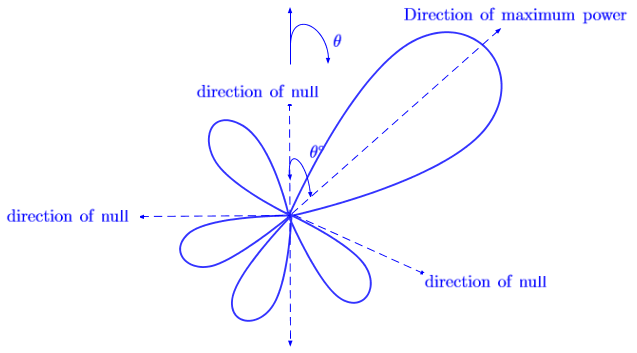
\includegraphics[height=5cm]{/graphics/maximum null}
\caption{Direction of nulls}
\label{figure8}
\end{figure}

The radiation pattern has a direction in which maximum power goes and five directions in which no power goes. Some important terms to note for a radiation pattern are:
\begin{enumerate}
\item [a]	An absolute maximum electric field is the electric field in the direction of the maximum power.
\item [b]	An electric field is said to be locally maximum if its magnitude(amplitude) is higher compared to the neighbouring points (the nulls) and its amplitude is smaller compared to the absolute maximum. In fig. \ref{figure8} there are four locally maximum electric fields.
\item [c]	The radiation pattern in the direction of the absolute maximum is called the main beam of the antenna, and
\item [d] 	The minor lobes where electric field is said to be locally maximum is called the side lobes.
\end{enumerate}

Therefore, our arbitrary radiation pattern is characterized by one main beam and four side lobes. We have discussed previously that depending on the application, the directional dependence of the antenna matters, just as we said before, if we desired a transfer of power in a particular direction then a highly directional antenna is used with characteristics of a narrow main beam and more nulls in the region where we are not transferring power and in another application, broadcasting application, we need power transfer in all directions which implies a wide beam with no nulls.
The radiation pattern can also be represented as a linear plot of the magnitude of electric field against direction $\theta$  as shown in Figure~\ref{figure9}
\begin{figure}[h]
\centering
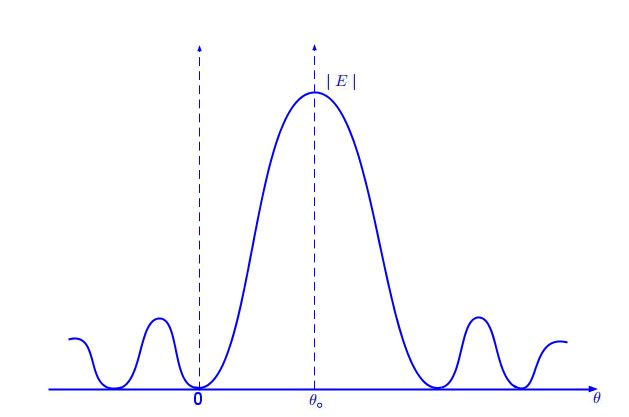
\includegraphics[height=5cm]{/graphics/sinc function1}
\caption{radiation pattern shown by linear plot of $|E|$ against $\theta$}
\label{figure9}
\end{figure}

Both the linear plot(or Cartesian plot) and the E-plane radiation pattern are used to analyze radiation patterns of an antenna.

Now let's take a look at the radiation characteristics as a basis for comparing antennas
\begin{enumerate}
\item[1]The first basic characteristic parameter that different antennas can be compared with is the \textbf{direction of the main beam ($\theta_\circ$, $\phi_\circ$)} for the three dimensional pattern with reference to an axis in the angular coordinate.

Let's now discuss the angular sector over which the main beam exists and consider a sector which radiates from the two nulls over which the power is propagating. We will have variations of electric field across the sector from maximum (at the tip of the main beam) to zero(at the nulls) which is very abrupt, so instead in electrical engineering we would prefer to consider a sector that spans an effective width such that the variation of power is 50\%. Hence, we want a sector that passes through a point on the beam where maximum power drops to 50\% of its maximum power and since P$\propto \mid E\mid^{2}$, then it is equivalent to the point on the beam when the magnitude of the electric field drops to $\frac{1}{\sqrt{2}}$ of its maximum value which is referred to as the 3dB points on the radiation pattern.

\begin{figure}[h]
\centering
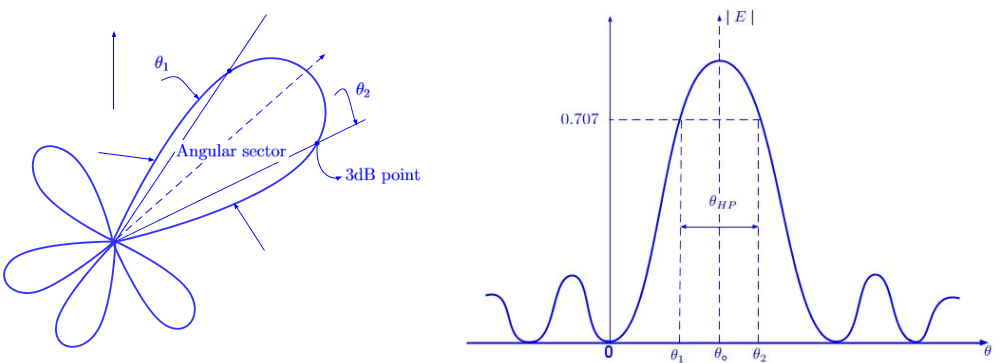
\includegraphics[width=1\linewidth]{/graphics/fig 10 new}
\label{figure10}
\end{figure}
\item[2]The next parameter is called the \textbf{half power beam width} and it is defined as the effective width over which the antenna is transferring power along the main beam; it is given by HPBW= $\theta_2 -\theta_1$.

It should be noted that the radiation pattern might not be circular in the H-plane so the effective sector does not form essentially a cone as is the case in the example. So for any shape of radiation pattern which is not a circle different planes are placed at the 3dB points with respect to the maximum point and then we get a HPBW that is varying. We recall that the 3 dimensional radiation pattern can be fully captured by the two principal planes; the E-plane and the H-plane. So for a radiation pattern which is not circular we would get the HPBW for the E-plane and the H-plane i.e. $\theta_{\textnormal{HP}}$ for E-plane and $\theta_{\textnormal{HP}}$ for H-plane. This parameter, the HPBW is a very important parameter and it is also often times called the 3dB beam-width.  

Also there is a third parameter which answers to the question of what is the effective angle over which the radiation goes? If we accept the variations of electric fields within the sector but provided radiation does not go to zero, the choice would be the first nulls on either sides of the main beam and then the beam width would be $\theta$ from Figure~\ref{figure11}

\begin{figure}[h]
\centering
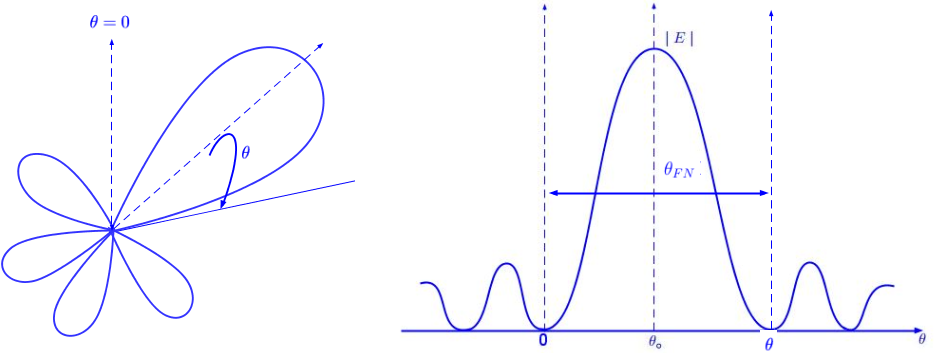
\includegraphics[width=1\linewidth]{/graphics/fig 11 new}
\label{figure11}
\end{figure}
\item[3]The third parameter is called the \textbf{beam width between first nulls}. It is denoted by BWFN; from Figure~\ref{figure11}, $\theta_{\textnormal{FN}}=\theta$. It is not a reliable quantity for description of effective power transfer, the half power beam width is a more reliable parameter instead.

For directional antennas, in addition to beam for maximum power transfer there are the side lobes which transfer power in the regions in its path which is very undesirable. In design of directional antenna these side lobes are reduced to minimum as possible and as such its level needs to be measured.
\item[4.]A good figure of merit to measure how much power would leak is the \textbf{side lobe level} which is the ratio of the highest amplitude value of the local maxima and the main beam amplitude given as;
$$ Side\ lobe\ level\ (SLL)=\frac{largest\ side\ lobe\ amplitude}{Main\ beam\ amplitude}(dB)$$
Since the main lobe amplitude is unity for normalized radiation pattern, essentially the amplitude of the largest side lobe defines the side lobe level.. Typically, the value for a good antenna lies between about -20 to -30dB.

The poynting vector as a parameter for measuring power is distance dependent and it is not useful for far fields. From the expression of the electric field, it varies as $\dfrac{1}{r}$ and power density P$\propto |E|^{2}$ means it is inversely proportional to to the square of  r and its value decreases as we move from the antenna. Hence, we would define another parameter which is not distance dependent called the \textbf{radiation intensity}.
\item[5.] The Radiation intensity U$(\theta, \phi)$ is the power per unit solid angle .

\begin{figure}[h]
\centering
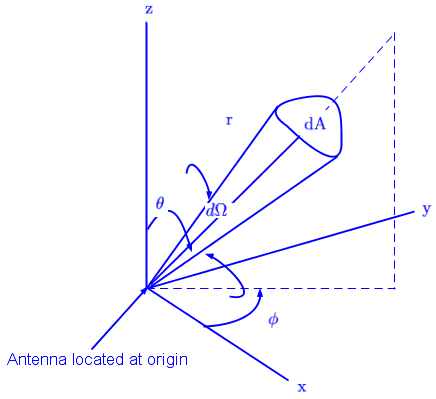
\includegraphics[height=5cm]{/graphics/fig 12 new}
\label{figure12}
\end{figure}
Solid angle, d$\Omega$ as shown in Figure~\ref{figure12} is an angle subtended by an area dA from the origin (source or antenna) given by;$$d\Omega=\frac{dA}{r^{2}};$$

for the spherical coordinate dA = $r^{2}\sin \theta d\theta d\phi$

So d$\Omega=\sin d\theta d\phi$

Radiation Intensity, $U(\theta ,\phi) = \frac{W(\theta,\phi)}{d\Omega}$

$$= \frac{W(\theta ,\phi)}{\frac{dA}{r^{2}}}$$

$$= \frac{W(\theta ,\phi)}{dA} r^{2}$$

Recall $\dfrac{W(\theta ,\phi)}{dA}$ is the power density which varies as $\dfrac{1}{r^{2}}$. So we see that the $r^{2}$ cancels and the radiation intensity $U(\theta ,\phi)$ is not a function of r or it is not distance dependent.
We know that the power density which is the poynting vector is given by: $\dfrac{1}{2}\dfrac{|E|^{2}}{\eta}$, so $U(\theta ,\phi)=\dfrac{1}{2}\frac{|E|^{2}}{\eta}r^{2}$\\
Next, we will determine a very important parameter called \textbf{directivity}.
\item[5.] Directivity is a measure of how directional an antenna is , it is the measure of the capability the antenna has in focusing power in a direction. Alternatively, it may be defined as measure of how much radiation intensity an antenna would produce in the direction of maximum radiation compared to that it would produce if the radiation were uniformly distributed in all directions. Or simply the ratio of the radiation intensity of the directional antenna to that of the isotropic antenna.
So essentially, directivity of an antenna  is maximum radiation intensity  divided by the average radiation intensity.

Power radiated by antenna,
\begin{align*}
W=\int_{4\pi}U(\theta ,\phi)d\Omega\\
 =\int_{\phi=0}^{2\pi}\int_{\theta=0}^{\pi}U(\theta,\phi)\sin\theta d\theta d\phi
\end{align*}

The average radiation intensity $U_{\textnormal{av}}$, is the power uniformly distributed in all directions. Mathematically;

$U_{\textnormal{av}}=\dfrac{1}{\textnormal{solid angle}} \times$ total power radiated

We would get the solid angle as 4$\pi$, if power is radiated in all directions, then it constitutes a sphere of surface area equal to $4\pi r^{2}$

Solid angle = $\dfrac{\text{Surface area}}{r^{2}} = 4\pi$

So, $U_{\textnormal{av}}=\frac{1}{4\pi} \times W = \frac{1}{4\pi}\int_{4\pi}U(\theta ,\phi)d\Omega$

Then, Directivity $D=\dfrac{U_{\textnormal{max
}}}{U_{\textnormal{av}}}$ 

\begin{equation}
= \frac{4\pi U_{\textnormal{max}}}{\int_{4\pi}U(\theta,\phi)d\Omega}
\label{eqn14}
\end{equation}

$U_{\textnormal{max}}$ is the maximum radiation intensity of the antenna under consideration and it is gotten from the radiation pattern:
$$U_{\textnormal{max}}=\frac{1}{2}\frac{|E|^{2}_{\textnormal{max}}r^{2}}{\eta}$$
$$U_{\textnormal{max}}=\frac{1}{2}\frac{|E(\theta,\phi)|^{2}r^{2}}{\eta}$$

Substituting into D in Equation~\ref{eqn14}

$$
D = \dfrac{4\pi\left\{\dfrac{r^2}{2}
	\dfrac{|E|^2_{max}}{\eta}\right\}}
{{\Large \int_{4\pi}}\dfrac{r^2}{2}
	\dfrac{|E(\theta,\phi)|^2}{\eta}d\Omega }
$$

\begin{equation}
D = \dfrac{4\pi|E|^2_{max}}{\int^{ 2\pi}_{\phi=0}\int^{ \pi}_{\theta=0}|E(\theta,\phi)|^2\sin\theta d\theta d\phi \qquad \quad}
\label{eqn14b}
\end{equation}
The above expression shows the directivity D is purely defined by the radiation pattern because $|E|_{max}$ and $|E(\theta, \phi)|$ can be gotten from the radiation pattern.

let's rewrite the Equation~\ref{eqn14b} with the normalized radiation pattern given as $\frac{E(\theta, \phi)}{|E|_{max}} = E_n$ then, Equation~\ref{eqn14b} becomes

\begin{equation}
D = \frac{4\pi}{\int_{\phi = 0}^{2\pi}\int_{\theta = 0}^{2\pi}|E_n(\theta, \phi)|^2\sin\theta d\theta d\phi}
\label{eqn14c}
\end{equation}

In conclusion if we know the normalized radiation pattern then we can calculate the directivity of a given antenna.
		
Directivity shows the enhancement of the radiation intensity in a given direction with respect to an isotropic antenna, so for an isotropic antenna the directivity is 1 but for a directional antenna the directivity is greater than one. Hence directivity is always greater than or equal to one $(D\geq 1)$.
For example, the satellite antennas, which are highly directional have very high directivity typically in the order of about $10^{5}-10^{6}$ and so have a very high focusing power.	Let's consider a case study for a very narrow beam i.e. $(\theta, \phi << 1rad)$ with a radiation pattern shown in Figure~\ref{figure16}. We will assume the power is effectively confined to the half power beam width.  

\begin{figure}[h]
\centering
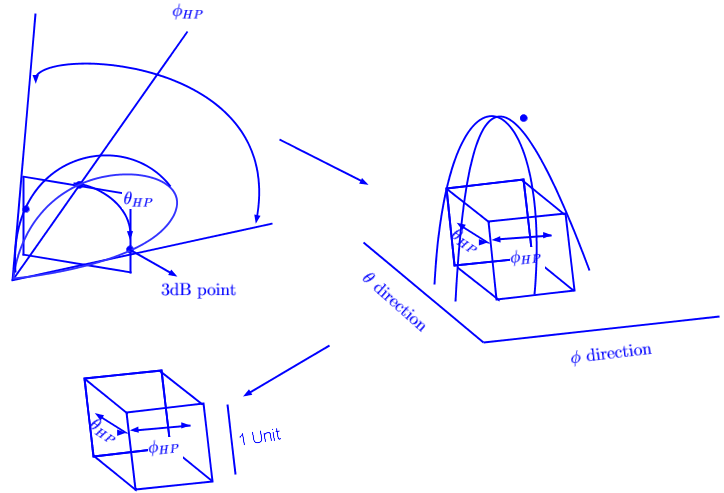
\includegraphics[height=5cm]{/graphics/fig 16 lec 47}
\label{figure16}
\end{figure}

Also we will assume the side lobe is much smaller for the antenna. The 3D radiation pattern is shown as well as 3D linear plot or (Cartesian plot) and we will consider two perpendicular planes which cut the 3D plot at the 3dB points. Then this points can be visualized like a box where the whole power is confined that has width $\theta_{\textnormal{HP}}$ and $\phi_{\textnormal{HP}}$. Therefore the denominator of Equation~\ref{eqn14c} which is $\int_{\phi=0}^{2\pi} \int_{\theta=0}^{\pi}|E_{\textnormal{n}}(\theta, \phi)|^{2}\sin\theta d\theta d\phi$ is approximately the box.
Since, the plot is a normalized radiation pattern, which means the amplitude is 1 so the height of the box is unity. Under the assumption that the angle is very small $(\theta_{HP}, \phi_{HP} \ll 1rad)$ then $\int_{\phi=0}^{2\pi} \int_{\theta=0}^{\pi}|E_{\textnormal{n}}(\theta, \phi)|^{2}\sin\theta d\theta d\phi$ is the volume of the box.

So, 
$$D \approx \dfrac{4\pi}{\theta_{\textnormal{HP}}\phi_{\textnormal{HP}}}$$
$$\approx \frac{4\pi}{\Omega}$$
where $\Omega$ is the beam solid angle given as $\Omega =\theta_{\textnormal{HP}}\phi_{\textnormal{HP}} $ .
This is the directivity of a very directional antenna and it is approximately measured with values of the HPBW.	
\end{enumerate}	
\begin{exmp}
Calculate the directivity of a parabolic dish whose main beam is circular that gives the half power beam width of $1^\circ$ by $1^\circ$.
\begin{center}
Solution
$\theta_{\textnormal{HP}} =\phi_{\textnormal{HP}} =1^{\circ
}=\dfrac{\pi}{180}$rad


$D=\dfrac{4\pi}{\theta_{\textnormal{HP}}\phi_{\textnormal{HP}}}$
$= \frac{4(180)^2}{\pi} \approx 40,000$
\end{center}
\end{exmp}

This means that at a given distance this antenna would enhance the radiation intensity by 40,000, this is why the directivity is sometimes called the gain of the antenna. Let's examine this closely, if we had distributed power uniformly we would have gotten a certain amount of power but by narrowing the distribution(using the parabolic dish) the power was enhanced by a factor of 40,000. Said differently, if we did not have this antenna and we wanted to produce this power density at a given distance we would require the power which is 40,000 times more than what is required if we used this antenna.

In conclusion, for point to point communication like microwave link or satellite communication, we use the antennas which are highly directional and this reduces the power capabilities of the communication link. The antenna (directional) provides the gain of the power, however this is not the same as the conventional sense of an amplifier. The antenna simply enhances power in a given direction at the expense of other directions which is not needed. The enhancement or amplification is not increase in total power which is radiated, the total power is conserved, all the directional antennas do is to redistribute power to a specific direction and then there is amplification of power. Therefore, directivity is a very important parameter and it plays an important role in reducing the power requirement in the communication link. Directivity as well as other characteristics discussed are important characteristics of an antenna when it is used as a transmitting antenna.